
\section{Classificatie en logistische regressie}

In het vorige hoofdstuk zijn we ingegaan op de vraag hoe we op basis van een bepaald aantal gegevens een voorspelling kunnen doen van de waarde van een ander gegeven – hoe, bijvoorbeeld, de waarde van een huis samenhangt met de grootte, of hoe de omzet van een vervoerder samenhangt met de stad waarin hij opereert. Een andere belangrijke tak van sport binnen machine learning betreft de zogenaamde \textit{classificatie-problematiek}, waarbij we observaties onderverdelen in een set van categorieën.

Een mooi voorbeeld van een dergelijk vraagstuk wordt gevormd door e-mails. Stel je voor dat we een aantal categorieën hebben waarin we onze binnenkomende e-mails onderverdelen: ongewenste reclame natuurlijk, maar ook werk-gerelateerd, privé of mails van onze vrienden. Kunnen we nu een systeem trainen dat op zoek gaat naar verschillende eigenschappen van die binnenkomende mail en op basis hiervan deze mail automatisch in de juiste categorie onderverdeelt? 

Meer algemeen kunnen we classificatie als volgt omschrijven: gegeven een set $X$ van $m$ observaties, kunnen we een systeem maken van voor een nieuwe observatie $x$ een hypothese $h(x)$ formuleert of deze observatie \textit{wel} ($y=1$) of \textit{niet} ($y=0$) tot een bepaalde categorie behoort? Een systeem dat hierover uitspraken doet wordt een \textit{classificeerder}(of in het Engels \textit{classifier}) genoemd.


\subsection{De sigmoïdefunctie}

In tegenstelling tot de eerdere problemen, wordt bij classificatie de mogelijke output dus beperkt tot nul of één. Hoewel er natuurlijk een grijs gebied is, kun je van de meeste e-mails wel direct zeggen of het evident spam is of niet. Om deze situatie te kunnen modelleren, moeten we dus een functie hebben die 0 heeft als laagste waarde, 1 als hoogste waarde en een relatief snelle overgang tussen deze twee. De functie die aan deze eigenschappen voldoet, is de \textit{sigmoïdefunctie}:

\[
g(z) = \frac{1}{1+e^{-z}}
\]

\begin{figure}[h]
\centering
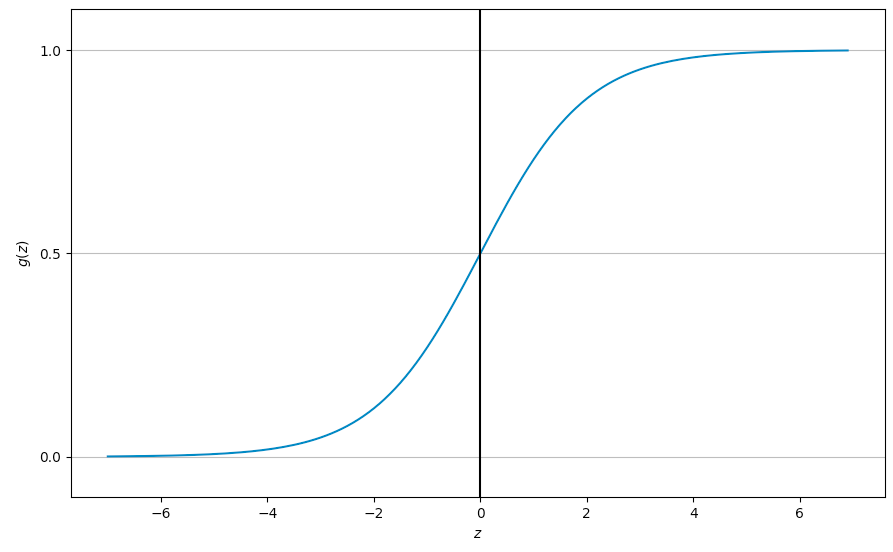
\includegraphics[width=.75\textwidth]{sigmoid}
\caption{De sigmoïdefunctie\label{img:sigmoid}}
\end{figure}

Zoals je in figuur \ref{img:sigmoid} ziet is in deze functie $y\approx1$ voor relatief hoge waarden van $x$, en $y\approx0$ voor relatief lage waarden van $x$. De functie gaat door het punt $(0,\frac{1}{2})$, want $e^0=1$. 

We gebruiken nu deze sigmoïdefunctie om de kans uit te rekenen of data tot een bepaalde categorie behoort of niet. Wanneer we bijvoorbeeld een lijst hebben van woorden die vaak in spam e-mails voorkomen, zouden we eenvoudig kunnen tellen hoe vaak deze woorden in een specifiek bericht voorkomen en op basis daarvan kunnen aangeven hoe \textit{waarschijnlijk} het is dat dit bericht een spam-bericht is. Stel nu dat we een bericht hebben waarin drie van dergelijke woorden voorkomen. Een berekening zou er dan als volgt uit kunnen zien:

%
\[
x = \begin{bmatrix}
x_0\\
x_1\\
\end{bmatrix}
= \begin{bmatrix}
1\\
aantalWoorden\\
\end{bmatrix}
= \begin{bmatrix}
1\\
3\\
\end{bmatrix}.
\]
%
Als we vervolgens stellen dat we hebben gevonden dat $\theta_0=-0,1$ en $\theta_1=-0,2$, dan geldt 
%
\[
\begin{aligned}
z &= \theta^Tx
= \begin{bmatrix}
-0,1 & -0,2\\
\end{bmatrix}
\begin{bmatrix}
1\\
3\\
\end{bmatrix} \\
&= -0,1 + -0,6 = -0,7.
\end{aligned}
\]
%
De waarschijnlijkheid dat dit bericht een spam-bericht is, wordt dan gegeven door 
%
\[
\begin{aligned}
h_\theta(x) &= g(\theta^Tx) = \frac{1}{1+e^{-z}}\\
&= \frac{1}{1+e^{0,7}}
\approx \frac{1}{1+2,01} \\
&\approx \frac{1}{3,01} \approx 0,33.
\end{aligned}
\]
%
Met deze gegevens is er dus een kans van zo'n drieëndertig procent dat het bericht in kwestie een spam-bericht is. De vraag is natuurlijk, net als bij de lineaire regressie, hoe we tot de waardes van $\theta$ komen.


\subsection{De kostenfunctie voor logistische regressie}
Net als bij lineaire regressie hebben we ook bij logistische regressie te maken met een trainingsset van $m$ observaties: $\{(x^{(1)}, y^{(1)}), (x^{(2)}, y^{(2)}), \hdots, (x^{(m)}, y^{(m)})\}$, waarbij $y \in \{0,1\}$ en $x \in \{x_0, x_1, \hdots, x_n\}$ (elke $x$ heeft $n$ eigenschappen en $x_0=1$). Voor elke $x^{(i)}$ is er een hypothese die aangeeft of deze observatie wel of niet tot de specifieke categorie behoort. Deze hypothese wordt gegeven door de sigmoïdefunctie:

\[
h_\theta(x^{(i)}) = \frac{1}{1+e^{\theta^Tx^{(i)}}}
\]

Wanneer onze hypothesefunctie gemodelleerd is met de sigmoïdefunctie, dan is het niet handig om voor de kostenfunctie de som van de gekwadrateerde afwijkingen te gebruiken. We krijgen dan namelijk een zeer complexe berekening waarvan niet te garanderen is dat deze ook daadwerkelijk te minimaliseren is. Daarom maken we in het geval van de sigmoïdefunctie gebruik van een andere kostenfunctie. Die kostenfunctie is onder te verdelen in twee situaties: één waarbij $y=0$ en één waarbij $y=1$. Omdat we weten dat één van deze twee gegarandeerd het geval is, kunnen we deze twee situaties met een wiskundig handigheidje tot één formule reduceren:

\[
\begin{aligned}
Kost(h_\theta(x), y) &= 
\begin{cases}
  -log(h_\theta(x)) & \text{als $y=1$} \\
  -log(1-h_\theta(x)) & \text{als $y=0$} \\
\end{cases}\\
&= -ylog(h_\theta(x)) - (1-y)log(1-h_\theta(x)).
\end{aligned}
\]

Wanneer we deze formule toepassen, zien we dat in het geval dat $h_\theta(x) \rightarrow 1$ en $y=1$ (wanneer we, kortom, correct voorspellen dat de observatie $x$ inderdaad tot deze specifieke categorie behoort) de \textit{kost} voor deze voorspelling nadert naar 0 ($log(1)=0$). Omgekeerd, wanneer $h_\theta(x) \rightarrow 0$ (terwijl $y=1$), nadert deze kost oneindig ($log(0)=-\infty$). Mutatis mutandis geldt hetzelfde voor de situatie wanneer $y=0$. Dit klopt natuurlijk ook met onze intuïtie: wanneer we een correcte voorspelling doen, willen we dat de kost van de hypothese die dat weergeeft minimaal is; als we een incorrecte voorspelling doen, is deze kost daarentegen erg hoog. Wanneer we nu de kosten voor alle observaties bij elkaar optellen en delen door het aantal observaties, dan krijgen we dus weer de gemiddelde kosten voor deze specifieke set van $\theta$:

\[
J(\theta) = \frac{1}{m}\sum_{i=1}^m \left[y^{(i)}log(h_\theta(x^{(i)})) + (1-y^{(i)})log(1-h_\theta(x^{(i)}))\right]
\]

Net als bij lineaire regressie is het nu het doel om deze kosten tot een minimum te reduceren. Om dit te bereiken moeten we weer de afgeleide van de formule hierboven hebben. Hoewel hij er wellicht indrukwekkend uitziet, is de afgeleide opvallend eenvoudig (en herkenbaar):

\[
\begin{aligned}
& \textrm{Herhaal tot een minimum is bereikt}\\
& \textrm{(gelijktijdige update voor alle $\theta_j$, $j=0 \hdots n$)}\{\\
& \theta_j := \theta_j - \alpha \frac{\partial}{{\partial}{\theta_j}}J(\theta) \\
& = \theta_j - \alpha \frac{1}{m}\sum_{i=1}^{m} (h_\theta(x^{(i)}) - y^{(i)})x_j^{(i)}\\
&\}.
\end{aligned}
\]

Kortom, de update-regel is voor logistische regressie hetzelfde als voor lineaire regressie. Het enige – belangrijke – verschil is dat we in het dit geval de sigmoïde-functie gebruiken om $h_\theta(x)$ uit te rekenen, terwijl we bij lineaire regressie een eenvoudige lijn gebruiken.

\subsection{Classificatie met meerdere klassen}
De methoden die we hierboven hebben beschreven, kunnen we gebruiken voor zogenaamde \textit{binaire classificatie}: een observatie behoort tot een bepaalde klasse toe of niet. Hoe kunnen we nu deze technieken gebruiken om data onder te verdelen in meerdere klassen, bijvoorbeeld om e-mails te sorteren op spam, werk-gerelateerd, privé of van vrienden? 

Stel je voor dat we een situatie hebben waarin we data willen onderverdelen in vier categorieën. Onze trainingsdata bevat in dat geval $y\in{0,1,2,3}$: voor elke observatie is hierin aangegeven tot welke categorie deze behoort. Op de manier die hierboven beschreven is, kunnen we voor elke categorie een separate classificeerder trainen, die een kans geeft of een observatie tot deze specifieke klasse behoort of niet. Wanneer we dan een nieuwe observatie hebben, kiezen we die classificeerder die de hoogste waarschijnlijkheid aangeeft.

Wanneer we te maken hebben met $m$ klassen, dan trainen we dus $m$ classificeerders die voor elke nieuwe observatie $(x^{(i)}, y^{(i)})$ aangeven hoe groot de kans is dat $y=m$. Zie ook figuur \ref{img:multiclass}, waarin de kans het grootst is dat de observatie behoort tot de derde klasse.

\begin{figure}[h]
\centering
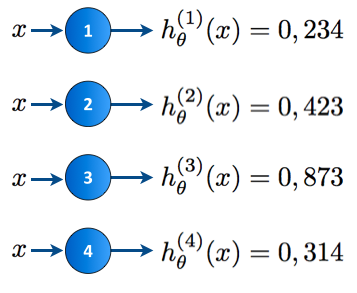
\includegraphics[width=.75\textwidth]{multiclass}
\caption{Classificatie over meerdere categorieën.\label{img:multiclass}}
\end{figure}

